%% LyX 2.4.4 created this file.  For more info, see https://www.lyx.org/.
%% Do not edit unless you really know what you are doing.
\documentclass[english,t]{beamer}
\usepackage{mathptmx}
\usepackage[T1]{fontenc}
\usepackage[latin9]{inputenc}
\usepackage{amssymb}
\usepackage{cancel}
\PassOptionsToPackage{normalem}{ulem}
\usepackage{ulem}

\makeatletter

%%%%%%%%%%%%%%%%%%%%%%%%%%%%%% LyX specific LaTeX commands.
%% Because html converters don't know tabularnewline
\providecommand{\tabularnewline}{\\}

%%%%%%%%%%%%%%%%%%%%%%%%%%%%%% Textclass specific LaTeX commands.
% this default might be overridden by plain title style
\newcommand\makebeamertitle{\frame{\maketitle}}%
% (ERT) argument for the TOC
\AtBeginDocument{%
  \let\origtableofcontents=\tableofcontents
  \def\tableofcontents{\@ifnextchar[{\origtableofcontents}{\gobbletableofcontents}}
  \def\gobbletableofcontents#1{\origtableofcontents}
}

%%%%%%%%%%%%%%%%%%%%%%%%%%%%%% User specified LaTeX commands.
\usetheme{Warsaw}
% or ...

\setbeamercovered{transparent}
% or whatever (possibly just delete it)
\setbeamercovered{invisible} %makes overlays invisible

%gets rid of navigation symbols
\setbeamertemplate{navigation symbols}{}

%\usepackage{hyperref}
%\usepackage[usenames,dvipsnames,table]{xcolor} %adds additional color options
\definecolor{links}{HTML}{2A1B81}
%\hypersetup{colorlinks,linkcolor=blue,urlcolor=links}

\usepackage{multicol}

\usepackage{tikz}
\usetikzlibrary{calc}
\usetikzlibrary{plotmarks}
\usetikzlibrary{shapes}
\usepackage{pgfplots}
\pgfplotsset{compat=newest}

\usepackage{forest} %%for tree diagram

\usepackage{calc}
\usepackage[nomessages]{fp}

%\usepackage{advdate}    % Advancing/saving dates
\usepackage{datetime}   % Dates formatting
%\usepackage{datenumber} % Counters for dates

\usepackage[super]{nth}

\usepackage{etex}

\usepackage{fancybox}

%%table colors
%\usepackage[table]{xcolor}
\usepackage{colortbl}

\usepackage[outline]{contour}  %allows text halos

\usepackage{epsdice} %%dice font
\usepackage[misc]{ifsym}
\newfont\dice{dice3d} %%3d dice font

\contourlength{1pt} %sets halo width
%%example: \node at (0.75,0.5) {\contour{white}{\Large Text!}};
%%example:  \node [fill=white,inner sep=1pt] at (2.25,0.5) {\Large 			Text!};
%%example:  \node [fill=white,rounded corners=2pt,inner sep=1pt] at 			(3.75,0.5) {\Large Text!};

%%%%%%%%%%%%%%%%%%%%%%%%%%%
\def\formatdateny{\csname noyear\languagename\expandafter\endcsname\formatdate}
\def\noyearenglish#1, \the\@year{#1}
\let\noyearamerican\noyearenglish
\let\noyearbritish\noyearenglish

%%allows uncover with forest diagrams
\tikzset{
    invisible/.style={opacity=0,text opacity=0},
    visible on/.style={alt=#1{}{invisible}},
    alt/.code args={<#1>#2#3}{%
      \alt<#1>{\pgfkeysalso{#2}}{\pgfkeysalso{#3}} % \pgfkeysalso doesn't change the path
    },
}
\forestset{
  visible on/.style={
    for tree={
      /tikz/visible on={#1},
      edge={/tikz/visible on={#1}}}}}

%%%redefines column alignment to match vertically
%\define@key{beamerframe}{t}[true]{% top
  %\beamer@frametopskip=.2cm plus .5\paperheight\relax%
  %\beamer@framebottomskip=0pt plus 1fill\relax%
 % \beamer@frametopskipautobreak=\beamer@frametopskip\relax%
  %\beamer@framebottomskipautobreak=\beamer@framebottomskip\relax%
  %\def\beamer@initfirstlineunskip{}%
%}

%%provides pdf with 4 slides per page; don't forget to add 'handout' to remove overlays
%\usepackage{pgfpages}
%\pgfpagesuselayout{4 on 1}[a4paper, landscape, border shrink=7mm]
%\pgfpageslogicalpageoptions{1}{border code=\pgfusepath{stroke}}
%\pgfpageslogicalpageoptions{2}{border code=\pgfusepath{stroke}}
%\pgfpageslogicalpageoptions{3}{border code=\pgfusepath{stroke}}
%\pgfpageslogicalpageoptions{4}{border code=\pgfusepath{stroke}}
%%%Don't forget to add 'handout'

\makeatother

\usepackage{babel}
\begin{document}
\newcommand{\xmax}{2000}
\newcommand{\xmin}{0}
\newcommand{\xstep}{0} %must be xmin+n
\newcommand{\ymax}{500}
\newcommand{\ymin}{0}
\newcommand{\ystep}{0} %must be ymin+n

\newcounter{countEx} \setcounter{countEx}{0}
\newcounter{countProb} \setcounter{countProb}{0}
\resetcounteronoverlays{countEx} \resetcounteronoverlays{countProb}

\newcommand{\ex}[3]{
	\addtocounter{countEx}{1}
	\only<#1-#2>{\begin{exampleblock} {Example \chNum.\secNum.\arabic{countEx}.} #3	\end{exampleblock}}
}

\newcommand{\prob}[4]{
	\addtocounter{countProb}{1}
	\only<#1-#2>{\begin{exampleblock} {Problem  \chNum.\secNum.\arabic{countProb}.\,#3} #4	\end{exampleblock}}
}

\newcommand{\yline}[4]{
	(#2 - #4)/(#1 - #3)*(x - #1) + #2
}

\beamerdefaultoverlayspecification{<+->}

%%%%Chapter and Section numbers%%%%%
\newcommand{\chNum}{3}
\newcommand{\secNum}{3}
\newcommand{\secTitle}{Basic Rules of Probability}
\date{\formatdate{8}{10}{2014} \& \formatdate{10}{10}{2014}}

\title[Section \chNum.\secNum: \secTitle]{Section \chNum.\secNum: \secTitle}

\subtitle{Finite Mathematics~~MTH 107~~Fall 2014}

\author{Dr.\,James Ashe}

\titlegraphic{\includegraphics[height=2.75cm]{/home/jim/JamesAshe/MHU/images/MarsHilUniversityLogo-Virtical.png}}

\institute{Mars Hill University}

\makebeamertitle 

%%True false command
\newcommand{\T}{\textcolor{green}{\contour{black}{T}}}
\newcommand{\F}{\textcolor{red}{\contour{black}{F}}}
\newcommand{\uT}[2]{\uncover<#1-#2>{\T}}
\newcommand{\uF}[2]{\uncover<#1-#2>{\F}}

%tkiz ball item 
\newcommand*\circled[1]{\tikz[baseline=(char.base)]
	{\node[circle,ball color=green!50!black!100, shade,   color=white,inner sep=1.2pt] (char) {\tiny #1};
	}
}
\begin{frame}{Review: 3.2}

\vspace{-.5cm}
\begin{columns}


\column{12cm}

\only<1-5>{
\begin{block}{Probability of an event, \$E\$}
The \emph{probability} of event $E$, denoted $p(E)$, is

\hfill \uncover<2->{$p(E)=\begin{array}{c}
\underline{{n(E)}}\\
n(S)
\end{array}$}%
\begin{tabular}{l}
\uncover<3->{\textcolor{red}{\footnotesize $\leftarrow$ number of ways $E$ can happen}}\tabularnewline
\uncover<4->{\textcolor{red}{\footnotesize $\leftarrow$ total number of outcomes}}\tabularnewline
\end{tabular}\hfill

if the experiment's outcomes are equally likely.
\end{block}
}

\only<6->{
\begin{block}{Odds of an event, \$E\$}
The \emph{odds} of event $E$, denoted $o(E)$, are

\uncover<7->{%
\begin{tabular}{crc}
 & $o(E)=n(E):n(E')$\uncover<9->{\textcolor{red}{\footnotesize $\leftarrow$ number of ways $E$ CANNOT happen}} & \tabularnewline
 & \uncover<8->{\textcolor{red}{\footnotesize  $\uparrow$ number of ways $E$ can happen}} \hspace{2.5cm} & \tabularnewline
\end{tabular}}

if the experiment's outcomes are equally likely.
\end{block}
}

\prob{5}{}{Find the following:}{A card is drawn from a 52 card deck. What is the probability of getting a queen of hearts?}

\vspace{.5cm}\prob{10}{}{Find the following:}{A card is drawn from a 52 card deck. What is the probability of getting a queen of hearts?}
\end{columns}
\end{frame}

\begin{frame}{Rules}

\begin{columns}


\column{5.5cm}
\begin{block}{Probability Rules}

\begin{enumerate}
\item <2->[1.] $p(\emptyset)=0$
\item <5->[2.] $p(S)=1$
\item <8->[3.] $0\leq p(E)\leq1$
\end{enumerate}
\end{block}
\only<3-11>{
\begin{itemize}
\item <3->Recall: $\emptyset=\{\,\,\}$, is the empty/null set.
\item <6->$S$, the \emph{sample space,} is set of all possible outcomes.
\item <9->$E$ is an event; $E\subseteq S$.
\end{itemize}
}

\column{5.5cm}

\vspace{10pt}
\begin{enumerate}
\item [1.]<4->$p(\emptyset)=\frac{n(\emptyset)}{n(S)}=\frac{0}{n(S)}=0$
\item [2.]<7->$p(S)=\frac{n(S)}{n(S)}=1$
\item [3.]<10->$0\leq n(E)\leq S$ so then 

\begin{enumerate}
\item []<11->$0\leq\frac{n(E)}{n(S)}\leq\frac{n(S)}{n(S)}=1$
\end{enumerate}
\end{enumerate}
\end{columns}
\end{frame}

\begin{frame}{Dice}

\vspace{-.5cm}
\begin{columns}


\column{5.5cm}

\ex{1}{}{A single six-sided dice is rolled. Find the probability
of:
\begin{itemize}
\item <4->[a.]$E_{1}$: a $7$ is rolled
\item <6->[b.]$E_{2}$: a number between $1$ and $6$ (inclusive) is rolled.
\item <8->[c.]$E_{3}$: a number between $1$ and $6$ is rolled.
\end{itemize}
}
\begin{block}{Probability Rules}

\begin{enumerate}
\item [1.] $p(\emptyset)=0$
\item [2.] $p(S)=1$
\item [3.] $0\leq p(E)\leq1$
\end{enumerate}
\end{block}

\column{5.5cm}

\uncover<2->{\dice{1}\dice{2}\dice{3}\dice{4}\dice{5}\dice{6}}

\uncover<3->{$S=\{1,2,3,4,5,6\}$}

\vspace{1pt}
\begin{itemize}
\item <5->[a.]$p(E_{1})=\frac{n(E_{1})}{n(S)}=\frac{0}{6}=0$ 
\item <7->[b.]$p(E_{2})=\frac{n(E_{2})}{n(S)}=\frac{6}{6}=6$
\item <9->[c.]$E_{3}=\{2,3,4,5\}$, so $n(E_{3})=4$

\begin{itemize}
\item <10->[]$p(E_{3})=\frac{n(E_{3})}{n(S)}=\frac{4}{6}=\frac{2}{3}$ 
\end{itemize}
\end{itemize}
\end{columns}
\end{frame}

\begin{frame}{Pairs of Dice}

\vspace{-.5cm}
\begin{columns}


\column{5.5cm}

\ex{1}{}{A pair of dice is rolled. Find the probability of:
\begin{itemize}
\item <2->[a.]$E_{1}$: a $7$ is rolled
\end{itemize}
}

\vspace{-.75cm} \begin{center} \uncover<6->{ \textcolor{black}{\dice{1}\dice{2}\dice{3}\dice{4}\dice{5}\dice{6}}}\\
\uncover<7->{$\times$}\\
\uncover<8->{ \textcolor{blue}{\dice{1}\dice{2}\dice{3}\dice{4}\dice{5}\dice{6}}}\\
\uncover<9->{$=36$ possibilities} \end{center}


\column{7cm}
\begin{itemize}
\item <3->[b.]Need to find:\\
\only<3-9>{$p(E_{1})=\begin{array}{c}
\underline{n(E_{1})}\\
n(S)
\end{array}$%
\begin{tabular}{l}
\uncover<5->{\textcolor{red}{\footnotesize $\leftarrow$ ways $E_{1}$ can occur}}\tabularnewline
\uncover<4->{\textcolor{red}{\footnotesize $\leftarrow$ total outcomes}}\tabularnewline
\end{tabular}}\only<10-22>{$p(E_{1})=\begin{array}{c}
\underline{n(E_{1})}\\
36
\end{array}$%
\begin{tabular}{l}
\uncover<5->{\textcolor{red}{\footnotesize $\leftarrow$ ways $E_{1}$ can occur}}\tabularnewline
\uncover<4->{\textcolor{red}{\footnotesize $\leftarrow$ total outcomes}}\tabularnewline
\end{tabular}}\only<23->{$p(E_{1})=\begin{array}{c}
\underline{6}\\
36
\end{array}=\begin{array}{c}
\underline{1}\\
6
\end{array}$}
\item []\only<12->{\dice{1}}\uncover<13->{$+$\textcolor{blue}{\dice{6}}$=7$}
\item []\only<14->{\dice{2}}\uncover<15->{$+$\textcolor{blue}{\dice{5}}$=7$}
\item []\only<16->{\dice{3}}\uncover<17->{$+$\textcolor{blue}{\dice{4}}$=7$}
\item []\only<17->{\dice{4}}\uncover<18->{$+$\textcolor{blue}{\dice{3}}$=7$}
\item []\only<19->{\dice{5}}\uncover<20->{$+$\textcolor{blue}{\dice{2}}$=7$}
\item []\only<21->{\dice{6}}\uncover<22->{$+$\textcolor{blue}{\dice{1}}$=7$}
\end{itemize}
\end{columns}
\end{frame}

\begin{frame}{Pairs of Dice}

\vspace{-.5cm}
\begin{columns}


\column{5cm}

\ex{1}{}{A pair of six-sided dice is rolled. Find the probability
of:
\begin{itemize}
\item <2->[b.]$E_{2}$: a $7$ or greater is rolled
\end{itemize}
}\vspace{.5cm} \uncover<5->{ \hspace{-.5cm}

\begin{tabular}{c|cccccc}
 & (1,\textcolor{blue}{1}) & (1,\textcolor{blue}{2}) & (1,\textcolor{blue}{3}) & (1,\textcolor{blue}{4}) & (1,\textcolor{blue}{5}) & (1,\textcolor{blue}{6})\tabularnewline
\textbf{2} & (2,\textcolor{blue}{1}) & (2,\textcolor{blue}{2}) & (2,\textcolor{blue}{3}) & (2,\textcolor{blue}{4}) & (2,\textcolor{blue}{5}) & (2,\textcolor{blue}{6})\tabularnewline
\textbf{3} & (3,\textcolor{blue}{1}) & (3,\textcolor{blue}{2}) & (3,\textcolor{blue}{3}) & (3,\textcolor{blue}{4}) & (3,\textcolor{blue}{5}) & (3,\textcolor{blue}{6})\tabularnewline
\textbf{4} & (4,\textcolor{blue}{1}) & (4,\textcolor{blue}{2}) & (4,\textcolor{blue}{3}) & (4,\textcolor{blue}{4}) & (4,\textcolor{blue}{5}) & (4,\textcolor{blue}{6})\tabularnewline
\textbf{5} & (5,\textcolor{blue}{1}) & (5,\textcolor{blue}{2}) & (5,\textcolor{blue}{3}) & (5,\textcolor{blue}{4}) & (5,\textcolor{blue}{5}) & (5,\textcolor{blue}{6})\tabularnewline
\textbf{6} & (6,\textcolor{blue}{1}) & (6,\textcolor{blue}{2}) & (6,\textcolor{blue}{3}) & (6,\textcolor{blue}{4}) & (6,\textcolor{blue}{5}) & (6,\textcolor{blue}{6})\tabularnewline
\cline{2-7}
\multicolumn{1}{c}{\textbf{7}} & \textbf{8} & \textbf{9} & \textbf{10} & \textbf{11} & \textbf{12} & \tabularnewline
\end{tabular}}

\column{6cm}
\begin{itemize}
\item <3->[a.]$p(E_{2})=\frac{n(E_{2})}{n(S)}$

\begin{itemize}
\item []<4-> \hspace{6pt}$=\frac{n(E_{2})}{36}$
\item []<6-> \hspace{6pt}$=\frac{21}{36}=\frac{7}{12}$
\end{itemize}
\end{itemize}
\end{columns}
\end{frame}

\begin{frame}{Pairs of Dice}

\vspace{-.5cm}
\begin{columns}


\column{5cm}

\ex{1}{}{A pair of six-sided dice is rolled. Find the probability
of:
\begin{itemize}
\item <2->[c.]$E_{3}$: Less than a $5$.
\end{itemize}
}\vspace{.5cm} \uncover<5->{ \hspace{-.5cm}

\begin{tabular}{c|cccccc}
 & (1,\textcolor{blue}{1}) & (1,\textcolor{blue}{2}) & (1,\textcolor{blue}{3}) & (1,\textcolor{blue}{4}) & (1,\textcolor{blue}{5}) & (1,\textcolor{blue}{6})\tabularnewline
\textbf{2} & (2,\textcolor{blue}{1}) & (2,\textcolor{blue}{2}) & (2,\textcolor{blue}{3}) & (2,\textcolor{blue}{4}) & (2,\textcolor{blue}{5}) & (2,\textcolor{blue}{6})\tabularnewline
\textbf{3} & (3,\textcolor{blue}{1}) & (3,\textcolor{blue}{2}) & (3,\textcolor{blue}{3}) & (3,\textcolor{blue}{4}) & (3,\textcolor{blue}{5}) & (3,\textcolor{blue}{6})\tabularnewline
\textbf{4} & (4,\textcolor{blue}{1}) & (4,\textcolor{blue}{2}) & (4,\textcolor{blue}{3}) & (4,\textcolor{blue}{4}) & (4,\textcolor{blue}{5}) & (4,\textcolor{blue}{6})\tabularnewline
\textbf{5} & (5,\textcolor{blue}{1}) & (5,\textcolor{blue}{2}) & (5,\textcolor{blue}{3}) & (5,\textcolor{blue}{4}) & (5,\textcolor{blue}{5}) & (5,\textcolor{blue}{6})\tabularnewline
\textbf{6} & (6,\textcolor{blue}{1}) & (6,\textcolor{blue}{2}) & (6,\textcolor{blue}{3}) & (6,\textcolor{blue}{4}) & (6,\textcolor{blue}{5}) & (6,\textcolor{blue}{6})\tabularnewline
\cline{2-7}
\multicolumn{1}{c}{\textbf{7}} & \textbf{8} & \textbf{9} & \textbf{10} & \textbf{11} & \textbf{12} & \tabularnewline
\end{tabular}}

\column{6cm}
\begin{itemize}
\item <3->[a.]$p(E_{3})=\frac{n(E_{3})}{n(S)}$

\begin{itemize}
\item []<4-> \hspace{6pt}$=\frac{n(E_{3})}{36}$
\item []<6-> \hspace{6pt}$=\frac{6}{36}=\frac{1}{6}$
\end{itemize}
\item []<7->Note: Not, $\frac{3}{12}$.
\item []<8-> \hspace{1cm}Also note,

\begin{itemize}
\item []<9-> \hspace{1cm}$P(\mbox{rolling }2)=\frac{1}{36}$\\
\hspace{1cm}$P(\mbox{rolling }3)=\frac{2}{36}$\\
\hspace{1cm}$p(\mbox{rolling }4)=\frac{3}{36}$
\item []<9-> \hspace{1cm}$\frac{1}{36}+\frac{2}{36}+\frac{3}{36}=\frac{6}{36}$
\end{itemize}
\end{itemize}
\end{columns}
\end{frame}

\begin{frame}{Mutually Exclusive Events}

\begin{block}{Mutually Exclusive Events}
To events that cannot occur at the same time are called \emph{mutually
exclusive}. 

\begin{itemize}
\item []<2->i.e., $E$ and $F$ are mutually exclusive \uline{if and only
if} $E\cap F=\emptyset$
\item <3->Recall: $E\cap F$ is the set of elements in \uline{both} $E$
\uline{and} $F$.
\end{itemize}
\end{block}
\begin{center}\only<1-3>{%%%%AnB=empty%%%%%
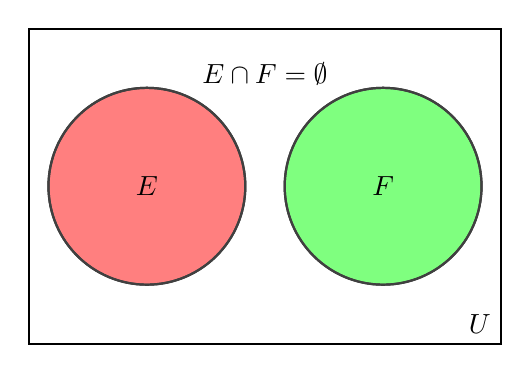
\begin{tikzpicture}[scale=1.0]
	\def\circleA{(-.5,0) circle (1.25)} %A
	\def\circleB{(2.5,0) circle (1.25)} %B

	\colorlet{circle edgeA}{black!75} 
	\colorlet{circle areaA}{red!100}
	\colorlet{circle edgeB}{black!75} 
	\colorlet{circle areaB}{green!100}

	\tikzset{
		filledA/.style={fill=circle areaA, draw=circle edgeA, thick},
		filledB/.style={fill=circle areaB, draw=circle edgeB, thick},
		outlineA/.style={draw=circle edgeA, thick},
		outlineB/.style={draw=circle edgeB, thick},
	}
	
	\begin{scope}[fill opacity=0.5]        
			\fill[filledB] \circleB;
			\fill[filledA] \circleA;
	\end{scope}

	\draw[outlineA] \circleA node {$E$}; 
	\draw[outlineB] \circleB node {$F$}; 
	\node[above=-3pt] at (current bounding box.north) {$E \cap F = \emptyset$}; 
	\draw[thick] (-2,-2) rectangle (4,2) node[anchor=south east] at (current bounding box.south east) {$U$}; 
\end{tikzpicture} } \only<4-4>{%%%%AUB-AnB%%%%%
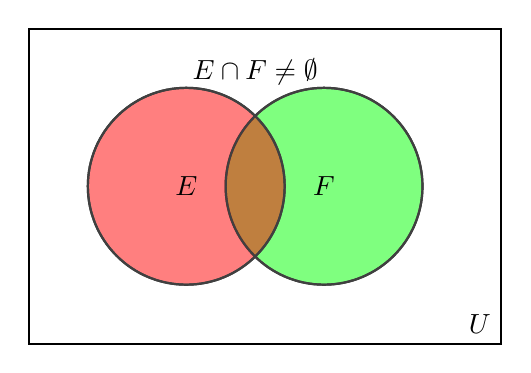
\begin{tikzpicture}[scale=1.0]
	\def\circleA{(0,0) circle (1.25)} %A
	\def\circleB{(1.75,0) circle (1.25)} %B

	\colorlet{circle edgeA}{black!75} 
	\colorlet{circle areaA}{red!100}
	\colorlet{circle edgeB}{black!75} 
	\colorlet{circle areaB}{green!100}

	\tikzset{
		filledA/.style={fill=circle areaA, draw=circle edgeA, thick},
		filledB/.style={fill=circle areaB, draw=circle edgeB, thick},
		outlineA/.style={draw=circle edgeA, thick},
		outlineB/.style={draw=circle edgeB, thick},
	}
	
	\begin{scope}[fill opacity=0.5]        
			\fill[filledB] \circleB;
			\fill[filledA] \circleA;
	\end{scope}

	\draw[outlineA] \circleA node {$E$}; 
	\draw[outlineB] \circleB node {$F$}; 
	\node[above=-3pt] at (current bounding box.north) {$E \cap F \neq \emptyset$}; 
	\draw[thick] (-2,-2) rectangle (4,2) node[anchor=south east] at (current bounding box.south east) {$U$}; 
\end{tikzpicture} }\only<5-5>{%%%%AnB=empty%%%%%
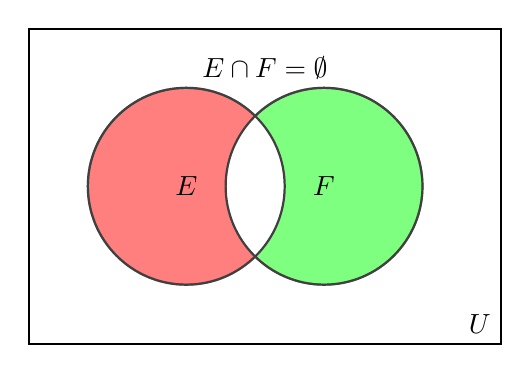
\begin{tikzpicture}[scale=1.0]
	\def\circleA{(0,0) circle (1.25)} %A
	\def\circleB{(1.75,0) circle (1.25)} %B

	\colorlet{circle edgeA}{black!75} 
	\colorlet{circle areaA}{red!100}
	\colorlet{circle edgeB}{black!75} 
	\colorlet{circle areaB}{green!100}

	\tikzset{
		filledA/.style={fill=circle areaA, draw=circle edgeA, thick},
		filledB/.style={fill=circle areaB, draw=circle edgeB, thick},
		outlineA/.style={draw=circle edgeA, thick},
		outlineB/.style={draw=circle edgeB, thick},
	}	       
		\begin{scope}[even odd rule,opacity=.5]% B-A             
			\clip \circleA (-2,-2) rectangle (4,2);
			\fill[filledB]\circleB;        
		\end{scope}
		\begin{scope}[even odd rule,opacity=.5]% A-B             
			\clip \circleB (-2,-2) rectangle (4,2);
			\fill[filledA]\circleA;        
		\end{scope}         	

	\draw[outlineA] \circleA node {$E$}; 
	\draw[outlineB] \circleB node {$F$}; 
	\draw[thick] (-2,-2) rectangle (4,2) node[anchor=south east] at (current bounding box.south east) {$U$}; 
	\node[below=7pt] at (current bounding box.north) {$E \cap F = \emptyset$}; 

\end{tikzpicture} }

\prob{6}{6}{Determine whether the two events are mutually exclusive}{
\begin{itemize}
\item [$E_{1}$:] Being a doctor.
\item [$E_{2}$:] Being a woman.
\end{itemize}
}

\prob{7}{7}{Determine whether the two events are mutually exclusive}{
\begin{itemize}
\item [$E_{1}$:] Being alive.
\item [$E_{2}$:] Being dead.
\end{itemize}
}

\prob{8}{8}{Determine whether the two events are mutually exclusive}{
\begin{itemize}
\item [$\heartsuit$:] Drawing a Heart (from a standard 52 card deck).
\item [$\spadesuit$:] Drawing a Spade.
\end{itemize}
}

\prob{9}{9}{Determine whether the two events are mutually exclusive}{
\begin{itemize}
\item [$J$:] Drawing a Jack (from a standard 52 card deck).
\item [$\spadesuit$:] Drawing a spade.
\end{itemize}
}

\end{center}
\end{frame}

\begin{frame}{Probability Rules}

\vspace{-.5cm}
\begin{columns}


\column{12cm}
\begin{block}{Probability Rules}

\begin{itemize}
\item [1.]<11->\only<11-11>{$n(A\cup B)=n(A)+n(B)-n(A\cap B)$.} \only<12->{$p(A\cup B)=p(A)+p(B)-p(A\cap B)$.}
\item [2.]<22->\only<22-22>{$n(A\cup B)=n(A)+n(B)$ if $A\cap B=\emptyset$.} \only<23->{$p(A\cup B)=p(A)+p(B)$
if $A\cap B=\emptyset$.}
\item [3.]<29->\only<30-30>{$n(A')=n(U)-n(A)$.} \only<31-31>{$p(A')=\frac{n(S)}{n(S)}-p(A)$.} \only<32->{$p(A')=1-p(A)$.}
\end{itemize}
\end{block}
\end{columns}
\only<1-12>{%
\noindent\begin{minipage}[t]{1\columnwidth}%
\ex{1}{12}{What is the probability of drawing a queen OR heart?}

\only<4->{$P(Q\cup H)=\frac{n(Q\cup H)}{n(S)}$\only<5->{$=\frac{n(Q\cup H)}{52}$}\only<10->{$=\frac{16}{52}=\frac{4}{13}$}}

\only<6->{$n(Q\cup H)=n(Q)+n(H)-n(Q\cap H)$$\leftarrow$\textbf{Union/Intersection
rule}}

\only<8->{$n(Q\cup H)=4+13$\only<9->{$-1$}}

\only<7-12>{
\begin{itemize}
\item []<2->$Q=\{q\clubsuit,q\spadesuit,q\heartsuit,q\diamondsuit\}$
\item []<3->$H=\{2\heartsuit,3\heartsuit,4\heartsuit,5\heartsuit,6\heartsuit,7\heartsuit,8\heartsuit,9\heartsuit,10\heartsuit,j\heartsuit,q\heartsuit,k\heartsuit,a\heartsuit\}$
\end{itemize}
}%
\end{minipage}}\only<13-23>{%
\noindent\begin{minipage}[t]{1\columnwidth}%
\ex{13}{23}{What is the probability of drawing a queen OR ace?}

\only<14->{$P(Q\cup A)=\frac{n(Q\cup A)}{n(S)}$\only<15->{$=\frac{n(Q\cup A)}{52}$}\only<20->{$=\frac{8}{52}$}}

\only<16->{$n(Q\cup A)=n(Q)+n(A)-n(Q\cap A)$}

\only<18->{$n(Q\cup A)=4+4$\only<19->{$-0$$\leftarrow$$Q\cap A=\emptyset$}}

\only<17->{
\begin{itemize}
\item []$Q=\{q\clubsuit,q\spadesuit,q\heartsuit,q\diamondsuit\}$
\item []$A=\{a\clubsuit,a\spadesuit,a\heartsuit,a\diamondsuit\}$
\end{itemize}
}%
\end{minipage}}

\ex{24}{}{What is the probability of NOT drawing a queen or ace?}

\only<25->{$P(\left(Q\cup A\right)')=\frac{n((Q\cup A)')}{n(S)}=\frac{n((Q\cup A)')}{52}$\only<26->{$=\frac{44}{52}$}}

\only<27->{$n(Q\cup A)=8$}

\only<28->{$n((Q\cup H))=52-8$\only<29->{$=44$}}
\end{frame}

\begin{frame}{Problems}

\vspace{-.75cm}
\begin{columns}


\column{5.5cm}

\ex{1}{}{A pair of six-sided dice is rolled. Find the probability
of rolling:
\begin{itemize}
\item <2->[a.]$E_{3}$: Less than a $5$.
\item <3->[b.]$E_{4}$: $5$ or greater.
\item <4->[c.]$E_{5}$: $5$ or $4$.
\item <5->[d.]$E_{6}$: Odd or $5$. 
\end{itemize}
}\vspace{.25cm}

\uncover<1->{

\begin{tabular}{c|cccccc}
 & (1,\textcolor{blue}{1}) & (1,\textcolor{blue}{2}) & (1,\textcolor{blue}{3}) & (1,\textcolor{blue}{4}) & (1,\textcolor{blue}{5}) & (1,\textcolor{blue}{6})\tabularnewline
\textbf{2} & (2,\textcolor{blue}{1}) & (2,\textcolor{blue}{2}) & (2,\textcolor{blue}{3}) & (2,\textcolor{blue}{4}) & (2,\textcolor{blue}{5}) & (2,\textcolor{blue}{6})\tabularnewline
\textbf{3} & (3,\textcolor{blue}{1}) & (3,\textcolor{blue}{2}) & (3,\textcolor{blue}{3}) & (3,\textcolor{blue}{4}) & (3,\textcolor{blue}{5}) & (3,\textcolor{blue}{6})\tabularnewline
\textbf{4} & (4,\textcolor{blue}{1}) & (4,\textcolor{blue}{2}) & (4,\textcolor{blue}{3}) & (4,\textcolor{blue}{4}) & (4,\textcolor{blue}{5}) & (4,\textcolor{blue}{6})\tabularnewline
\textbf{5} & (5,\textcolor{blue}{1}) & (5,\textcolor{blue}{2}) & (5,\textcolor{blue}{3}) & (5,\textcolor{blue}{4}) & (5,\textcolor{blue}{5}) & (5,\textcolor{blue}{6})\tabularnewline
\textbf{6} & (6,\textcolor{blue}{1}) & (6,\textcolor{blue}{2}) & (6,\textcolor{blue}{3}) & (6,\textcolor{blue}{4}) & (6,\textcolor{blue}{5}) & (6,\textcolor{blue}{6})\tabularnewline
\cline{2-7}
\multicolumn{1}{c}{\textbf{7}} & \textbf{8} & \textbf{9} & \textbf{10} & \textbf{11} & \textbf{12} & \tabularnewline
\end{tabular}}

\column{6cm }

\end{columns}
\end{frame}

\begin{frame}{Problems}

\prob{1}{1}{A card is randomly dealt from a standard 52 card deck. Find the probability that the card is as stated.}{
\begin{itemize}
\item [a.]A jack and red.
\item [b.]A jack or red.
\item [c.]Not a red jack.
\end{itemize}
}

\prob{2}{2}{A card is randomly dealt from a standard 52 card deck. Find the probability that the card is as stated.}{
\begin{itemize}
\item [a.]A 5 and a black.
\item [b.]A 5 or a black.
\item [c.]Not a black 5.
\end{itemize}
}
\end{frame}

\begin{frame}{Problems}

\prob{1}{1}{Find the relative frequency with which a customer's bill is as stated.}{
\begin{itemize}
\item [a.]Less than \$80.00.
\item [b.]\$80.00 or more.
\end{itemize}
}

\prob{2}{2}{Find the relative frequency with which a customer's bill is as stated.}{
\begin{itemize}
\item [a.]Between \$40.00 and \$79.99.
\item [b.]Not between \$40.00 and \$79.99.
\end{itemize}
}
\begin{columns}


\column{6cm}

\begin{tabular}{|c|c|}
\hline 
\rowcolor{yellow!50}\textbf{Size of Bill} & \textbf{\# of Customers}\tabularnewline
\hline 
\hline 
below \$20 & 200\tabularnewline
\hline 
\$20-39.99 & 100\tabularnewline
\hline 
\$40-59.99 & 150\tabularnewline
\hline 
\$60-79.99 & 50\tabularnewline
\hline 
\$80-99.99 & 300\tabularnewline
\hline 
above \$100 & 100\tabularnewline
\hline 
\end{tabular}

\column{5cm}

\end{columns}
\end{frame}

\begin{frame}{Probabilities and Venn Diagrams}

\vspace{-.5cm}
\begin{columns}


\column{5.5cm}

\ex{1}{}{The probability that a student \emph{passes} Art is 75\%,
\emph{fails} Math is 65\%, and \emph{passes} at least one is 85\%.
Find that a student:
\begin{itemize}
\item [a.]passes Math.
\item <5->[b.]passes both.
\item <11->[c.]fails both.
\item <15->[d.]passes only one. 
\end{itemize}
}

\column{5.5cm}

\vspace{.5cm}\only<2-2>{%%%%M'%%%%%
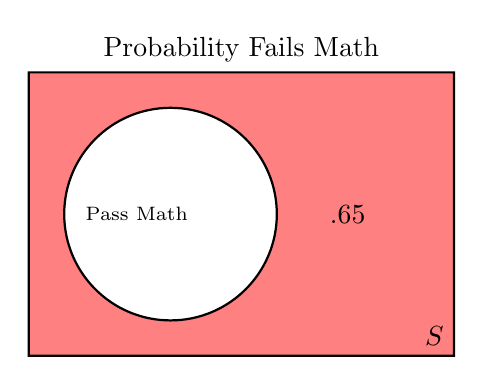
\begin{tikzpicture}[scale=.9]
	\def\circleA{(0,0) circle (1.5)} %A
	\def\circleB{(0:2) circle (1.5)} %B

	\colorlet{circle edgeA}{black!75} 
	\colorlet{circle areaA}{red!100}
	\colorlet{circle edgeB}{black!75} 
	\colorlet{circle areaB}{blue!100}

	\tikzset{
		filledA/.style={fill=circle areaA, draw=circle edgeA, thick},
		filledB/.style={fill=circle areaB, draw=circle edgeB, thick},
		outlineA/.style={draw=circle edgeA, thick},
		outlineB/.style={draw=circle edgeB, thick},
	}

	\draw[thick,fill=red!50,even odd rule] %%even odd rule draws compliment of next draw commands%%
		(-2,-2) rectangle (4,2) node[anchor=south east] at (current bounding box.south east) {$S$} 
		\circleA node[left=-10pt] {\scriptsize Pass Math} node[below=2pt] {};
	\node[anchor=south] at (current bounding box.north) {Probability Fails Math}; 
	\node at (2.5,0) {.65};	

\end{tikzpicture} } \only<3-3>{%%%% M %%%%%
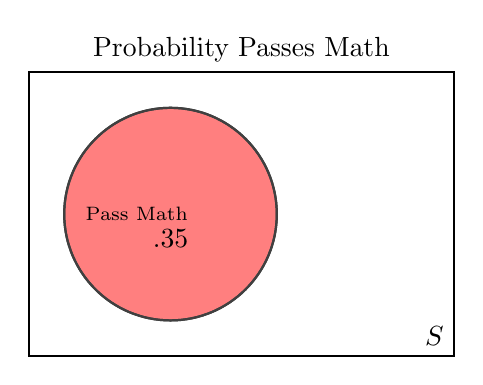
\begin{tikzpicture}[scale=.9]
	\def\circleA{(0,0) circle (1.5)} %A
	\def\circleB{(0:2) circle (1.5)} %B

	\colorlet{circle edgeA}{black!75} 
	\colorlet{circle areaA}{red!100}
	\colorlet{circle edgeB}{black!75} 
	\colorlet{circle areaB}{green!100}

	\tikzset{
		filledA/.style={fill=circle areaA, draw=circle edgeA, thick},
		filledB/.style={fill=circle areaB, draw=circle edgeB, thick},
		outlineA/.style={draw=circle edgeA, thick},
		outlineB/.style={draw=circle edgeB, thick},
	}
	
	\begin{scope}[fill opacity=0.5]         
			\fill[filledA] \circleA;
			%\fill[filledB] \circleB;    
	\end{scope}

	\draw[outlineA] \circleA node[left=-10pt] {\scriptsize Pass Math} node[below=2pt] {.35}; 
	%\draw[outlineB] \circleB node[right=-10pt] {\scriptsize Pass Art}; 
	\draw[thick] (-2,-2) rectangle (4,2) node[anchor=south east] at (current bounding box.south east) {$S$}; 
	\node[anchor=south] at (current bounding box.north) {Probability Passes Math}; 
\end{tikzpicture} }

 \only<4-8>{%%%% M or A %%%%%
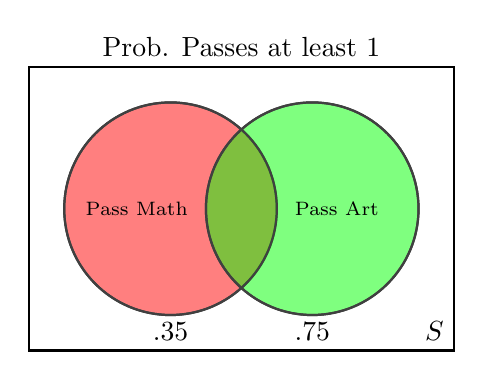
\begin{tikzpicture}[scale=.9]
	\def\circleA{(0,0) circle (1.5)} %A
	\def\circleB{(0:2) circle (1.5)} %B

	\colorlet{circle edgeA}{black!75} 
	\colorlet{circle areaA}{red!100}
	\colorlet{circle edgeB}{black!75} 
	\colorlet{circle areaB}{green!100}

	\tikzset{
		filledA/.style={fill=circle areaA, draw=circle edgeA, thick},
		filledB/.style={fill=circle areaB, draw=circle edgeB, thick},
		outlineA/.style={draw=circle edgeA, thick},
		outlineB/.style={draw=circle edgeB, thick},
	}
	
	\begin{scope}[fill opacity=0.5]         
			\fill[filledA] \circleA;
			\fill[filledB] \circleB;    
	\end{scope}

	\draw[outlineA] \circleA node[left=-10pt] {\scriptsize Pass Math} node[below=-1pt] at (0,-1.5) {.35}; 
	\draw[outlineB] \circleB node[right=-10pt] {\scriptsize Pass Art} node[below=-1pt] at (2,-1.5) {.75};
	%\draw (1,0) node {.25};
	\draw[thick] (-2,-2) rectangle (4,2) node[anchor=south east] at (current bounding box.south east) {$S$}; 
	\node[anchor=south] at (current bounding box.north) {Prob. Passes at least 1}; 
\end{tikzpicture} } \only<9-9>{%%%% M and A %%%%%
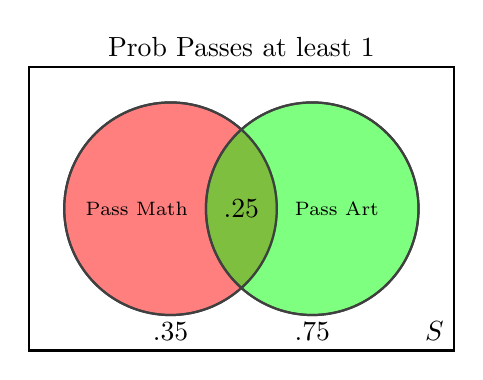
\begin{tikzpicture}[scale=.9]
	\def\circleA{(0,0) circle (1.5)} %A
	\def\circleB{(0:2) circle (1.5)} %B

	\colorlet{circle edgeA}{black!75} 
	\colorlet{circle areaA}{red!100}
	\colorlet{circle edgeB}{black!75} 
	\colorlet{circle areaB}{green!100}

	\tikzset{
		filledA/.style={fill=circle areaA, draw=circle edgeA, thick},
		filledB/.style={fill=circle areaB, draw=circle edgeB, thick},
		outlineA/.style={draw=circle edgeA, thick},
		outlineB/.style={draw=circle edgeB, thick},
	}
	
	\begin{scope}[fill opacity=0.5]         
			\fill[filledA] \circleA;
			\fill[filledB] \circleB;    
	\end{scope}

	\draw[outlineA] \circleA node[left=-10pt] {\scriptsize Pass Math} node[below=-1pt] at (0,-1.5) {.35}; 
	\draw[outlineB] \circleB node[right=-10pt] {\scriptsize Pass Art} node[below=-1pt] at (2,-1.5) {.75};
	\draw (1,0) node {.25};
	\draw[thick] (-2,-2) rectangle (4,2) node[anchor=south east] at (current bounding box.south east) {$S$}; 
	\node[anchor=south] at (current bounding box.north) {Prob Passes at least 1}; 
\end{tikzpicture} }\only<10-10>{%%%%MnA%%%%%
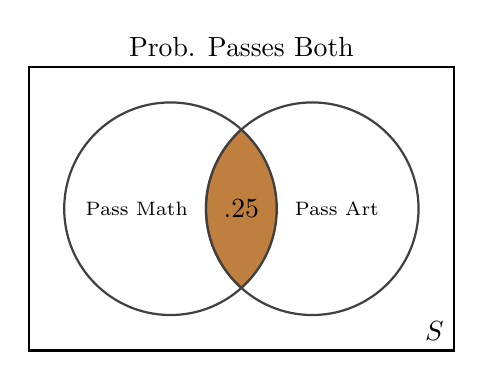
\begin{tikzpicture}[scale=.9]
	\def\circleA{(0,0) circle (1.5)} %A
	\def\circleB{(0:2) circle (1.5)} %B

	\colorlet{circle edgeA}{black!75} 
	\colorlet{circle areaA}{red!100}
	\colorlet{circle edgeB}{black!75} 
	\colorlet{circle areaB}{green!100}

	\tikzset{
		filledA/.style={fill=circle areaA, draw=circle edgeA, thick},
		filledB/.style={fill=circle areaB, draw=circle edgeB, thick},
		outlineA/.style={draw=circle edgeA, thick},
		outlineB/.style={draw=circle edgeB, thick},
	}
	
	\begin{scope}[fill opacity=0.5]    
		\clip \circleA;     
			\fill[filledB] \circleB;
		\clip \circleB;     
			\fill[filledA] \circleA;
	\end{scope}

	\draw[outlineA] \circleA node[left=-10pt] {\scriptsize Pass Math} node[below=-1pt] at (0,-1.5) {}; 
	\draw[outlineB] \circleB node[right=-10pt] {\scriptsize Pass Art} node[below=-1pt] at (2,-1.5) {};
	\draw (1,0) node {.25};

	%\node[anchor=south] at (current bounding box.north) {$A \cap B$}; 
	\draw[thick] (-2,-2) rectangle (4,2) node[anchor=south east] at (current bounding box.south east) {$S$};
	\node[anchor=south] at (current bounding box.north) {Prob. Passes Both};
\end{tikzpicture} }\only<11-14>{%%%%(MUA)' complement%%%%%
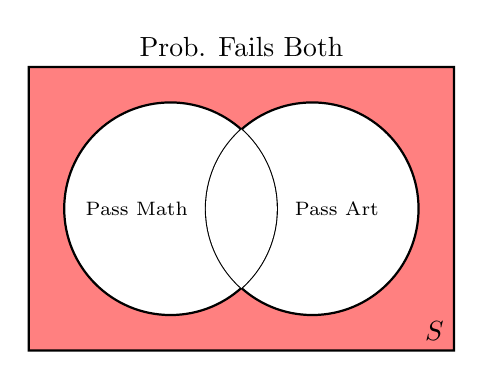
\begin{tikzpicture}[scale=.9]
	\def\circleA{(0,0) circle (1.5)} %A
	\def\circleB{(0:2) circle (1.5)} %B

	\colorlet{circle edgeA}{black!75} 
	\colorlet{circle areaA}{red!100}
	\colorlet{circle edgeB}{black!75} 
	\colorlet{circle areaB}{blue!100}

	\tikzset{
		filledA/.style={fill=circle areaA, draw=circle edgeA, thick},
		filledB/.style={fill=circle areaB, draw=circle edgeB, thick},
		outlineA/.style={draw=circle edgeA, thick},
		outlineB/.style={draw=circle edgeB, thick},
	}

		\draw[thick,fill=red!50,even odd rule] %%even odd rule draws complement of next draw commands%%
			(-2,-2) rectangle (4,2) node[anchor=south east] at (current bounding box.south east) {$S$}
			\circleA node[left=-10pt] {\scriptsize Pass Math} node[below=-1pt] at (0,-1.5) {}
			\circleB node[right=-10pt] {\scriptsize Pass Art} node[below=-1pt] at (2,-1.5) {};

		\scope 
			\clip (0,0) circle (1.5);%%why can't i use circleA?
			\fill[white] (0:2) circle (1.5); 
		\endscope
		
	\node[anchor=south] at (current bounding box.north) {Prob. Fails Both}; 

\end{tikzpicture} } \only<17-18>{%%%% M %%%%%
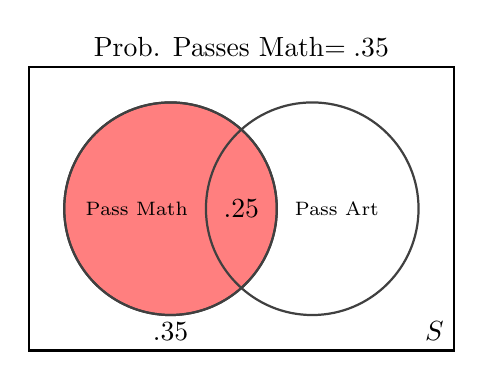
\begin{tikzpicture}[scale=.9]
	\def\circleA{(0,0) circle (1.5)} %A
	\def\circleB{(0:2) circle (1.5)} %B

	\colorlet{circle edgeA}{black!75} 
	\colorlet{circle areaA}{red!100}
	\colorlet{circle edgeB}{black!75} 
	\colorlet{circle areaB}{green!100}

	\tikzset{
		filledA/.style={fill=circle areaA, draw=circle edgeA, thick},
		filledB/.style={fill=circle areaB, draw=circle edgeB, thick},
		outlineA/.style={draw=circle edgeA, thick},
		outlineB/.style={draw=circle edgeB, thick},
	}
	
	\begin{scope}[fill opacity=0.5]         
			\fill[filledA] \circleA;
			%\fill[filledB] \circleB;    
	\end{scope}

	\draw[outlineA] \circleA node[left=-10pt] {\scriptsize Pass Math} node[below=-1pt] at (0,-1.5) {.35}; 
	\draw[outlineB] \circleB node[right=-10pt] {\scriptsize Pass Art} node[below=-1pt] at (2,-1.5) {};
	%\node[anchor=south] at (current bounding box.north) {$A \cup B$};
	\draw (1,0) node {.25};
	\draw[thick] (-2,-2) rectangle (4,2) node[anchor=south east] at (current bounding box.south east) {$S$};
	\node[anchor=south] at (current bounding box.north) {Prob. Passes Math$=.35$};
\end{tikzpicture} }\only<19-19>{%%%%M-A%%%%%
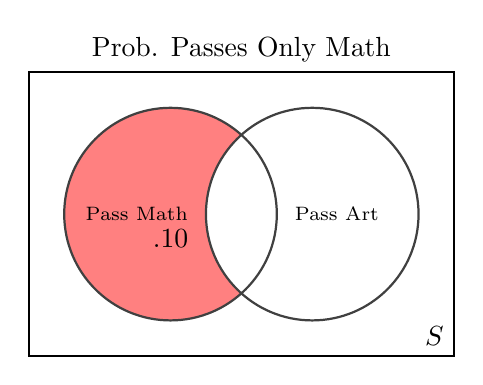
\begin{tikzpicture}[scale=.9]
	\def\circleA{(0,0) circle (1.5)} %A
	\def\circleB{(0:2) circle (1.5)} %B

	\colorlet{circle edgeA}{black!75} 
	\colorlet{circle areaA}{red!50}
	\colorlet{circle edgeB}{black!75} 
	\colorlet{circle areaB}{red!50}

	\tikzset{
		filledA/.style={fill=circle areaA, draw=circle edgeA, thick},
		filledB/.style={fill=circle areaB, draw=circle edgeB, thick},
		outlineA/.style={draw=circle edgeA, thick},
		outlineB/.style={draw=circle edgeB, thick},
	}
	
	\begin{scope}[fill opacity=1.0]    
		\fill[circle areaA] \circleA;
		\clip \circleA;     
			\fill[white] \circleB;
		%\clip \circleB;     
			%\fill[filledA] \circleA;
	\end{scope}

	\draw[outlineA] \circleA node[left=-10pt] {\scriptsize Pass Math} node[below=2pt] {.10}; 
	\draw[outlineB] \circleB node[right=-10pt] {\scriptsize Pass Art} node[below=-1pt] at (2,-1.5) {}; 
	\draw[thick] (-2,-2) rectangle (4,2) node[anchor=south east] at (current bounding box.south east) {$S$}; 
	\node[anchor=south] at (current bounding box.north) {Prob. Passes Only Math}; 
\end{tikzpicture} }\only<20-21>{%%%%A-M%%%%%
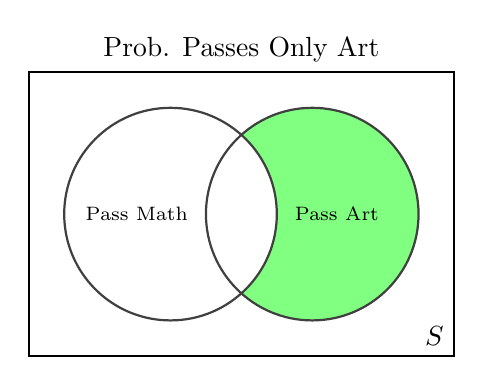
\begin{tikzpicture}[scale=.9]
	\def\circleA{(0,0) circle (1.5)} %A
	\def\circleB{(0:2) circle (1.5)} %B

	\colorlet{circle edgeA}{black!75} 
	\colorlet{circle areaA}{red!50}
	\colorlet{circle edgeB}{black!75} 
	\colorlet{circle areaB}{green!50}

	\tikzset{
		filledA/.style={fill=circle areaA, draw=circle edgeA, thick},
		filledB/.style={fill=circle areaB, draw=circle edgeB, thick},
		outlineA/.style={draw=circle edgeA, thick},
		outlineB/.style={draw=circle edgeB, thick},
	}
	
	\begin{scope}[fill opacity=1.0]    
		\fill[circle areaB] \circleB;
		\clip \circleA;     
			\fill[white] \circleB;
		%\clip \circleB;     
			%\fill[filledA] \circleA;
	\end{scope}

	\draw[outlineA] \circleA node[left=-10pt] {\scriptsize Pass Math} node[below=-1pt] at (0,-1.5) {}; 
	\draw[outlineB] \circleB node[right=-10pt] {\scriptsize Pass Art} node[below=2pt] {}; 
	\draw[thick] (-2,-2) rectangle (4,2) node[anchor=south east] at (current bounding box.south east) {$S$}; 
	\node[anchor=south] at (current bounding box.north) {Prob. Passes Only Art}; 
\end{tikzpicture} }\only<22->{%%%%(AuM)-(AnM)%%%%%
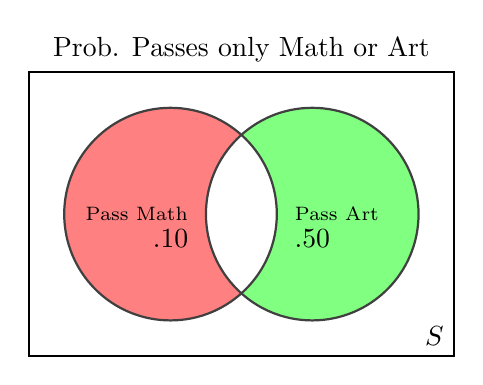
\begin{tikzpicture}[scale=.9]
	\def\circleA{(0,0) circle (1.5)} %A
	\def\circleB{(0:2) circle (1.5)} %B

	\colorlet{circle edgeA}{black!75} 
	\colorlet{circle areaA}{red!50}
	\colorlet{circle edgeB}{black!75} 
	\colorlet{circle areaB}{green!50}

	\tikzset{
		filledA/.style={fill=circle areaA, draw=circle edgeA, thick},
		filledB/.style={fill=circle areaB, draw=circle edgeB, thick},
		outlineA/.style={draw=circle edgeA, thick},
		outlineB/.style={draw=circle edgeB, thick},
	}
	
	\begin{scope}[fill opacity=1.0]    
		\fill[circle areaB] \circleB;
		\clip \circleA;     
			\fill[white] \circleB;
		%\clip \circleB;     
			%\fill[filledA] \circleA;
	\end{scope}

	\begin{scope}[fill opacity=1.0]    
		\fill[circle areaA] \circleA;
		%\clip \circleA;     
			%\fill[white] \circleB;
		\clip \circleB;     
			\fill[white] \circleA;
	\end{scope}

	\draw[outlineA] \circleA node[left=-10pt] {\scriptsize Pass Math} node[below=2pt] {.10}; 
	\draw[outlineB] \circleB node[right=-10pt] {\scriptsize Pass Art} node[below=2pt] {.50};  
	\draw[thick] (-2,-2) rectangle (4,2) node[anchor=south east] at (current bounding box.south east) {$S$}; 
	\node[anchor=south] at (current bounding box.north) {Prob. Passes only Math or Art}; 
\end{tikzpicture} }
\end{columns}
\vspace{.25cm}

\only<2-3>{Probability that a student does NOT fail Math: $1-.65$} \only<3-3>{$=.35$}

\only<5-9>{Probability that a student passes Math AND Art is: $P(M\cap A)$}

\only<6-10>{

\begin{tabular}{cccccccc}
\only<6->{ \textcolor{red}{Pass both$\downarrow$}} &  &  &  &  &  &  & \tabularnewline
$P(M\cup A)$ & $=$ & $P(M)$ & $+$ & $P(A)$ & $-$ & $P(M\cap A)$ & \tabularnewline
\only<6->{.85} & \only<6->{$=$} & \only<7->{$.35$} & \only<7->{$+$} & \only<8->{$.75$} & \only<8->{$-$} & \only<9->{$.25$} & \tabularnewline
\end{tabular}}\only<12-14>{Probability that a student does NOT pass at least
one.

\only<13-14>{ \hspace{1.5cm}$1-.85$} \only<14-14>{$=.15$}}

\only<16->{Probability that a student passes just Math} \only<20->{OR
just Art}

\only<17-19>{%
\begin{tabular}{ccccc}
$P(M)$ & $-$ & $P(M\cap A)$ &  & \tabularnewline
\only<18->{.35} & \only<18->{$-$} & \only<18->{.25} & \only<19->{$=.10$} & \tabularnewline
\end{tabular}}

\only<20-22>{%
\begin{tabular}{ccccc}
$P(A)$ & $-$ & $P(M\cap A)$ &  & \tabularnewline
\only<21->{.75} & \only<21->{$-$} & \only<21->{.25} & \only<21->{$=.5$} & \tabularnewline
\end{tabular}}

\only<23->{$.10+.50$} \only<24->{$=.60$}
\end{frame}

\end{document}
